\chapter{Derivados dos ácidos carboxílicos}\label{ch:b2:acyl-substitution}

Ferva azeite de oliva com hidróxido de sódio e você obtém sabão e glicerol: a
mais antiga reação orgânica conduzida de propósito. O óleo é um éster do
glicerol e de ácidos de cadeia longa, e o hidróxido corta cada éster em uma
única ligação, sempre a mesma, entre o carbono carbonílico e o oxigênio do
álcool. Ésteres, ácidos, amidas, anidridos e \omterm{def:b2:acyl-substitution:derivative}{cloretos de acila} reagem todos
assim: um nucleófilo se adiciona ao carbono carbonílico, e um grupo sai.
Classificar esses compostos pela facilidade com que seu grupo sai diz quais
podem ser transformados em quais, e em que sentido o químico precisa subir a
ladeira.

\begin{recall}
O volume do 1.º ano: ativação eletrofílica de um grupo carbonila, os mecanismos de formação dos
hemiacetais e acetais, adições de organomagnesianos, doadores de hidreto e seu alcance, grupos de
saída, $\mathrm pK_a$, $Q$ e $K$. \Cref{ch:b2:amines}: \omterm{def:b2:amines:nucleophilic-addition}{adição nucleofílica}, aminas.
\Cref{ch:b2:equilibrium-shifts}: deslocar um equilíbrio. O volume escolar: ésteres, ácidos
carboxílicos e amidas.
\end{recall}

\begin{omfigure}
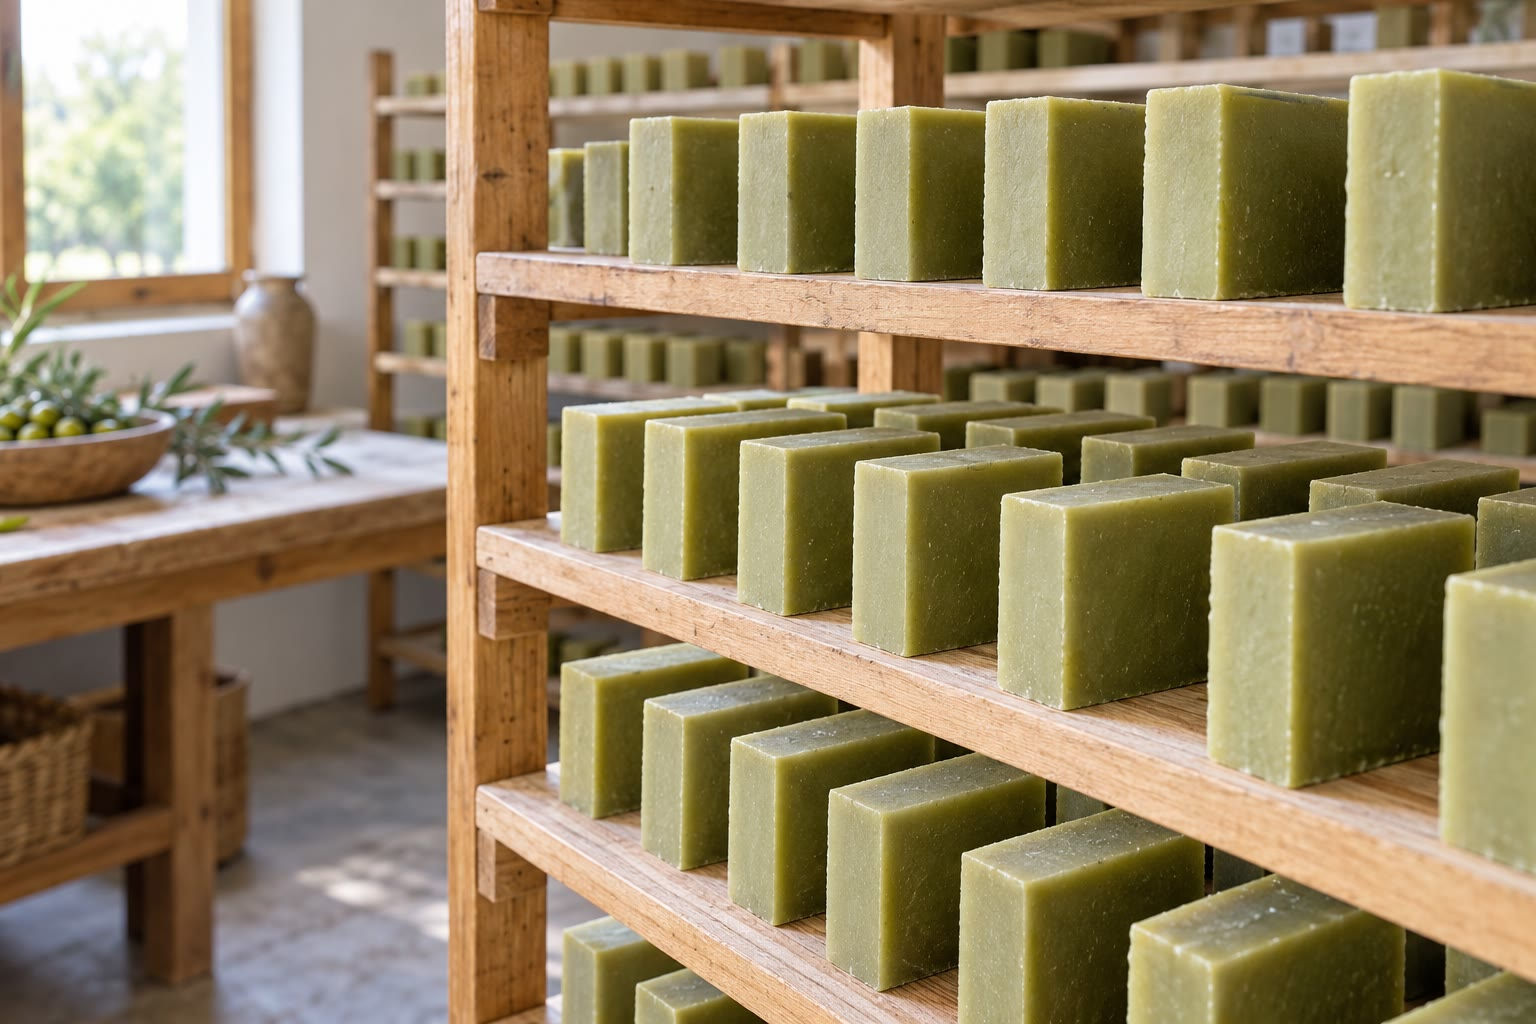
\includegraphics[width=0.58\linewidth]{images/book3/ai/b2-24-soap-bars.jpg}

{\small Barras de sabão de azeite secando em prateleiras de madeira. O sabão é o sal de sódio dos
ácidos graxos liberados quando o óleo, um éster, é fervido com hidróxido de sódio.}
\end{omfigure}

\section{A família e sua reatividade}

\begin{definition}[Derivados dos ácidos carboxílicos]\label{def:b2:acyl-substitution:derivative}
Um \emph{derivado de ácido carboxílico}\index{derivado de acido carboxilico@derivado de ácido carboxílico} é um composto \ce{R-CO-Z} no
qual o \ce{OH} de um ácido carboxílico é substituído por outro grupo Z. O \emph{grupo
acila}\index{grupo acila} $\mathrm{R{-}CO{-}}$ é comum a todos eles. Em um \emph{cloreto de acila}\index{cloreto de acila},
Z é Cl; em um \emph{anidrido de ácido}\index{anidrido de acido@anidrido de ácido}, Z é $\mathrm{O{-}CO{-}R'}$, dois grupos acila
compartilhando um oxigênio; em um éster Z é $\mathrm{OR'}$, em uma amida $\mathrm{NR'_2}$.
\end{definition}

\begin{proposition}[Escala de reatividade]\label{prop:b2:acyl-substitution:reactivity}
Diante dos nucleófilos, os derivados reagem na ordem \omterm{def:b2:acyl-substitution:derivative}{cloreto de acila} $>$ anidrido $>$ éster
$\approx$ ácido $>$ amida.
\end{proposition}

\begin{proof}[Raciocínio]
Dois efeitos se somam. O grupo de saída \ce{Z-} sai tanto mais facilmente quanto mais fraca é a
base que ele é: \ce{Cl-} (ácido conjugado \ce{HCl}, $\mathrm pK_a$ cerca de $-7$) muito melhor que
um carboxilato ($\mathrm pK_a$ cerca de 5), um alcóxido (cerca de 16) ou um íon amideto (cerca de
35). E o grupo Z doa densidade eletrônica à carbonila por doação mesomérica de seu par não
ligante, o que torna o carbono carbonílico menos eletrofílico: fraca para Cl, máxima para o
nitrogênio. A amida é ao mesmo tempo o eletrófilo mais fraco e o pior grupo de saída.
% ledger: pka:ethanoic, pka:ethanol
\end{proof}

\section{Substituição nucleofílica acílica}

\begin{definition}[Substituição nucleofílica acílica]\label{def:b2:acyl-substitution:nas}
Uma \emph{substituição nucleofílica acílica}\index{substituicao nucleofilica acilica@substituição nucleofílica acílica} substitui o grupo Z
de um composto acílico por um nucleófilo. Ela procede por adição do nucleófilo ao carbono
carbonílico, dando um \emph{intermediário tetraédrico}\index{intermediario tetraedrico@intermediário tetraédrico}, seguida da
eliminação do grupo de saída, que restabelece a ligação \ce{C=O}.
\end{definition}

\begin{proposition}[Adição--eliminação]\label{prop:b2:acyl-substitution:addition-elimination}
A substituição acílica passa por um \omterm{def:b2:acyl-substitution:nas}{intermediário tetraédrico}; ela é acelerada em meio básico por um
nucleófilo mais forte e em meio ácido pela ativação da carbonila.
\end{proposition}

\begin{proof}[Raciocínio]
O carbono carbonílico, plano e eletrofílico, recebe o nucleófilo por cima ou por baixo de seu
plano, como nas adições do \cref{ch:b2:amines}; com um grupo Z capaz de sair, o intermediário
o expulsa em vez de ser protonado. Em meio básico o nucleófilo é um ânion (\ce{HO-},
\ce{RO-}); em meio ácido o oxigênio carbonílico é protonado e um nucleófilo neutro (a água, um
álcool) basta. Ésteres marcados com \ce{^{18}O} na parte álcool dão, na hidrólise, álcool marcado
e ácido não marcado: a ligação rompida é a ligação acila--oxigênio, como o mecanismo exige.
\end{proof}

\begin{omfigure}
\setchemfig{atom sep=1.7em}
\schemestart
\chemfig{R-C(=[2]O)-OR'} \+ \chemfig{HO^{-}}
\arrow{->[adição]}
\chemfig{R-C(-[2]O^{-})(-[6]OH)-OR'}
\arrow{->[eliminação]}[,1.3]
\chemfig{R-C(=[2]O)-OH} \+ \chemfig{^{-}OR'}
\schemestop

\medskip
\setchemfig{arrow coeff=2.2}
\schemestart
\chemfig{R-C(=[2]O)-OH} \+ \chemfig{^{-}OR'}
\arrow{->[transferência de próton]}
\chemfig{R-C(=[2]O)-O^{-}} \+ \chemfig{HOR'}
\schemestop
\par\vspace{6pt}

{\small \omterm{def:b2:acyl-substitution:saponification}{Saponificação} de um éster. O hidróxido se adiciona ao carbono carbonílico, dando o
\omterm{def:b2:acyl-substitution:nas}{intermediário tetraédrico}; o alcóxido sai e a ligação \ce{C=O} se refaz; o alcóxido, uma base
forte, toma então o próton do ácido. Esta última etapa torna a reação completa.}
\end{omfigure}

\begin{method}[Desenhar uma substituição acílica]\label{met:b2:acyl-substitution:nas-mechanism}
\begin{enumerate}
  \item Em meio básico: o nucleófilo aniônico se adiciona ao carbono carbonílico; a carga negativa
        vai para o oxigênio; a ligação \ce{C=O} se refaz e Z sai; termine com uma eventual etapa
        ácido--base.
  \item Em meio ácido: protone o oxigênio carbonílico; o nucleófilo neutro se adiciona; transfira um
        próton ao grupo de saída; ele sai como molécula neutra; desprotone a carbonila.
  \item Conte as etapas: cada intermediário é ou tetraédrico ou um composto carbonílico.
\end{enumerate}
\end{method}

\section{Os ésteres}

\begin{definition}[Esterificação]\label{def:b2:acyl-substitution:esterification}
Uma \emph{esterificação}\index{esterificacao@esterificação} forma um éster a partir de um ácido carboxílico (ou de
um derivado mais reativo) e de um álcool. A reação direta de um ácido com um álcool, catalisada por
um ácido forte, é a esterificação de Fischer.
\end{definition}

\begin{proposition}[Esterificação de Fischer]\label{prop:b2:acyl-substitution:fischer}
A \omterm{def:b2:acyl-substitution:esterification}{esterificação} de Fischer é um equilíbrio lento, com constante perto de 4 para os álcoois
primários; ela é deslocada no sentido direto por um excesso de um reagente ou pela remoção da água à
medida que se forma.
\end{proposition}

\begin{proof}[Raciocínio]
Etanol e ácido etanoico equimolares param quando dois terços do ácido estão esterificados: $K =
(2/3)^2/(1/3)^2 = 4$. Com $Q < K$ mantido por um excesso de álcool, ou destilando a água
(o Dean--Stark do volume do 1.º ano), a reação avança mais
(\cref{ch:b2:equilibrium-shifts}). As seis etapas do mecanismo são as do \cref{met:b2:acyl-substitution:nas-mechanism}
em meio ácido, todas reversíveis.
% ledger: ester:berthelot
\end{proof}

\begin{definition}[Saponificação]\label{def:b2:acyl-substitution:saponification}
Uma \emph{saponificação}\index{saponificacao@saponificação} é a hidrólise de um éster por um hidróxido, dando
o sal carboxilato e o álcool.
\end{definition}

\begin{proposition}[A saponificação é completa]\label{prop:b2:acyl-substitution:saponification}
A \omterm{def:b2:acyl-substitution:saponification}{saponificação} é completa: sua última etapa, a transferência de próton do ácido carboxílico ao
alcóxido, tem uma constante de equilíbrio da ordem de $10^{11}$.
\end{proposition}

\begin{proof}
Para $\mathrm{RCOOH + R'O^- \to RCOO^- + R'OH}$,
\[
  K = \frac{K_a(\ce{RCOOH})}{K_a(\mathrm{R'OH})} = 10^{\mathrm pK_a(\mathrm{R'OH}) - \mathrm pK_a(\ce{RCOOH})} ;
\]
com o ácido etanoico (4.76) e o etanol (15.93), $K = 10^{11.2}$. O carboxilato, um eletrófilo fraco, não é atacado pelo álcool: a reação
global não volta atrás.
% ledger: pka:ethanoic, pka:ethanol
\end{proof}

\begin{omfigure}
\setchemfig{atom sep=1.7em}
\schemestart
\chemfig{CH_2(-[0]O-CO-R)-[6]CH(-[0]O-CO-R)-[6]CH_2-[0]O-CO-R}
\+ \chemfig{3\,NaOH}
\arrow{->[aquecimento]}
\chemfig{CH_2(-[0]OH)-[6]CH(-[0]OH)-[6]CH_2-[0]OH}
\+ \chemfig{3\,R-COO^{-}\,Na^{+}}
\schemestop
\par\vspace{6pt}

{\small \omterm{def:b2:acyl-substitution:saponification}{Saponificação} de um triglicerídeo: as três ligações éster são cortadas, dando o glicerol e
três moléculas do carboxilato de sódio, o sabão (R uma cadeia longa, \ce{C17H33} para o oleato do
azeite).}
\end{omfigure}

\begin{definition}[Transesterificação]\label{def:b2:acyl-substitution:transesterification}
Uma \emph{transesterificação}\index{transesterificacao@transesterificação} troca a parte álcool de um éster,
$\mathrm{RCOOR' + R''OH \rightleftharpoons RCOOR'' + R'OH}$, sob catálise ácida ou básica.
\end{definition}

\begin{definition}[Lactonas e lactamas]\label{def:b2:acyl-substitution:lactone}
Uma \emph{lactona}\index{lactona} é um éster cíclico, formado por \omterm{def:b2:acyl-substitution:esterification}{esterificação} interna de um
hidroxiácido; uma \emph{lactama}\index{lactama} é uma amida cíclica.
\end{definition}

\section{Os derivados ativados}

Descer a escala de reatividade é fácil: um \omterm{def:b2:acyl-substitution:derivative}{cloreto de acila} dá um anidrido, um éster ou uma
amida com o nucleófilo certo, muitas vezes à temperatura ambiente. Subir exige uma ativação: um
ácido carboxílico é transformado em seu cloreto pelo cloreto de tionila,
\[
  \ce{RCOOH + SOCl2 -> RCOCl + SO2 + HCl} ,
\]
cujos subprodutos são gases. O \omterm{def:b2:acyl-substitution:derivative}{cloreto de acila} reage então com um álcool ou uma amina; uma base
(piridina, trietilamina ou um segundo equivalente da amina) captura o \ce{HCl} formado, que
de outro modo protonaria a amina.

\begin{method}[Percorrer os derivados]\label{met:b2:acyl-substitution:ladder}
\begin{enumerate}
  \item Descendo a escala (cloreto $\to$ anidrido $\to$ éster, ácido $\to$ amida): trate com o
        nucleófilo, com uma base para captar o ácido liberado.
  \item Subindo a escala: converta primeiro o ácido no cloreto (\ce{SOCl2}); um éster ou uma amida
        é primeiro hidrolisado ao ácido.
  \item Entre um ácido e um éster: \omterm{def:b2:acyl-substitution:esterification}{esterificação} de Fischer (equilíbrio) ou \omterm{def:b2:acyl-substitution:saponification}{saponificação}
        (completa) seguida de acidificação.
\end{enumerate}
\end{method}

\begin{omfigure}
\begin{tikzpicture}[font=\small, >={Stealth}]
  \foreach \y/\n in {4/{cloreto de acila \ce{RCOCl}}, 3/{anidrido \ce{(RCO)2O}}, 2/{éster $\mathrm{RCOOR'}$ \quad ácido \ce{RCOOH}}, 1/{amida $\mathrm{RCONR'_2}$}} {
    \node[cyclenode, minimum width=5.2cm] at (0,\y*1.1) {\n};
  }
  \draw[->, thick, omDef] (-3.1,4.3) -- (-3.1,1.1) node[midway, left, align=right, font=\scriptsize] {fácil:\\ nucleófilo\\ + base};
  \draw[->, thick, omThm] (3.1,2.2) -- (3.1,4.4) node[midway, right, align=left, font=\scriptsize] {subida:\\ pelo ácido\\ e \ce{SOCl2}};
  \node[font=\scriptsize, anchor=south] at (0,4.85) {mais reativo};
  \node[font=\scriptsize, anchor=north] at (0,0.55) {menos reativo};
\end{tikzpicture}

{\small A escada de reatividade dos derivados dos ácidos carboxílicos. Qualquer derivado pode ser
transformado em um situado abaixo dele por um nucleófilo; subir passa pelo ácido e seu cloreto.}
\end{omfigure}

\section{Organometálicos e hidretos}

\begin{proposition}[Duas adições de Grignard]\label{prop:b2:acyl-substitution:grignard-ester}
Um éster tratado com excesso de reagente organomagnesiano dá um álcool terciário que leva dois
grupos idênticos vindos do reagente.
\end{proposition}

\begin{proof}[Raciocínio]
A primeira adição dá um \omterm{def:b2:acyl-substitution:nas}{intermediário tetraédrico} que expulsa o alcóxido: uma cetona. Uma cetona
é mais eletrofílica que um éster (sem doação mesomérica de um grupo $\mathrm{OR'}$) e reage com
o reagente mais depressa que o éster restante; a segunda adição, à cetona, dá o alcóxido
de um álcool terciário, que o tratamento ácido protona. A reação não pode ser parada na cetona.
\end{proof}

\begin{proposition}[Reduções por hidretos]\label{prop:b2:acyl-substitution:hydrides}
O hidreto de lítio e alumínio reduz ésteres e ácidos a álcoois primários, e amidas a aminas; o
boro-hidreto de sódio reduz aldeídos e cetonas, mas não ésteres, ácidos ou amidas. Um hidreto de
alumínio volumoso (DIBAL-H) a \qty{-78}{\degreeCelsius} reduz um éster ao aldeído.
\end{proposition}

\begin{proof}[Raciocínio]
\ce{LiAlH4} é um doador de hidreto forte: como o reagente de Grignard, ele se adiciona duas vezes
a um éster (passando pelo aldeído). O boro-hidreto é fraco demais para a carbonila de éster, menos
eletrofílica. Com DIBAL-H a baixa temperatura, o \omterm{def:b2:acyl-substitution:nas}{intermediário tetraédrico}, preso pelo alumínio,
não expulsa o alcóxido até o tratamento aquoso, quando já não resta hidreto: o aldeído sobrevive.
Em uma amida, é o oxigênio, ligado ao alumínio, que é eliminado em vez do nitrogênio, deixando um
íon imínio que o hidreto reduz à amina.
\end{proof}

\begin{history}[Chevreul e as gorduras]
\begin{minipage}[t]{0.22\linewidth}
\vspace{0pt}
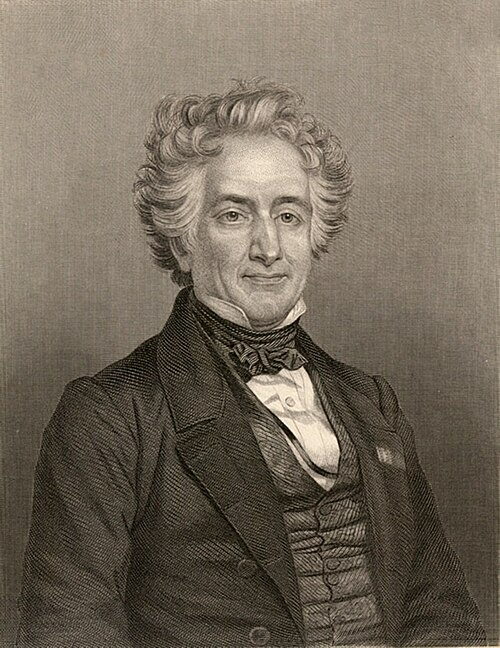
\includegraphics[width=\linewidth]{images/book3/chevreul.jpg}
\end{minipage}\hfill
\begin{minipage}[t]{0.74\linewidth}
\vspace{0pt}
Michel Eugène Chevreul mostrou, em um estudo publicado em 1823, que as gorduras são compostos do
glicerol com ácidos graxos, que ele isolou e nomeou (ácidos esteárico, oleico, butírico), e que a
\omterm{def:b2:acyl-substitution:saponification}{saponificação} as separa nessas duas partes. Seu trabalho transformou a fabricação de sabão e de
velas em química; ele viveu até os 102 anos. (Retrato por Nicolas Eustache Maurin, domínio
público, Wikimedia Commons.)
\end{minipage}
\end{history}

\begin{safety}{\ghs[5mm]{GHS02}\,\ghs[5mm]{GHS05}\,\ghs[5mm]{GHS06}}
O cloreto de tionila e os \omterm{def:b2:acyl-substitution:derivative}{cloretos de acila} reagem violentamente com a água e liberam gases
corrosivos; eles são manuseados a seco, na capela. O hidreto de lítio e alumínio inflama em contato
com a água; seu excesso é destruído com cuidado no final. O hidróxido de sódio concentrado é
corrosivo para a pele e os olhos. O metanol é tóxico e inflamável.
% ledger: ghs:SOCl2, ghs:ethanoyl-chloride, ghs:LiAlH4, ghs:NaOH, ghs:methanol
\end{safety}

\section{Exercícios}

\begin{exercise}[$\star$]\label{exo:b2:acyl-substitution:1}
Ordene por reatividade diante da água: etanoato de etila, cloreto de etanoíla, etanamida, anidrido
etanoico.
\end{exercise}

\begin{exercise}[$\star$]\label{exo:b2:acyl-substitution:2}
Dê os produtos do cloreto de etanoíla com: água; etanol; amônia (2 equivalentes);
etanoato de sódio; dimetilamina com trietilamina.
\end{exercise}

\begin{exercise}[$\star$]\label{exo:b2:acyl-substitution:3}
Escreva a \omterm{def:b2:acyl-substitution:saponification}{saponificação} do benzoato de metila pelo hidróxido de sódio e calcule a massa de
hidróxido de sódio necessária para \qty{13.6}{g} do éster.
\end{exercise}

\begin{exercise}[$\star$]\label{exo:b2:acyl-substitution:4}
Desenhe a \omterm{def:b2:acyl-substitution:lactone}{lactona} formada pelo ácido 4-hidroxibutanoico e dê o tamanho de seu anel.
\end{exercise}

\begin{exercise}[$\star\star$]\label{exo:b2:acyl-substitution:5}
Escreva o mecanismo da reação do etanoato de etila com a amônia.
\end{exercise}

\begin{exercise}[$\star\star$]\label{exo:b2:acyl-substitution:6}
A aspirina é preparada a partir do ácido salicílico (ácido 2-hidroxibenzoico) e do anidrido
etanoico. Que grupo do ácido salicílico reage, e qual é o subproduto?
\end{exercise}

\begin{exercise}[$\star\star$]\label{exo:b2:acyl-substitution:7}
O etanoato de etila é tratado com excesso de brometo de metilmagnésio e depois com ácido diluído.
Dê o produto e explique por que a cetona não pode ser isolada.
\end{exercise}

\begin{exercise}[$\star\star$]\label{exo:b2:acyl-substitution:8}
Dê o produto da redução da \omterm{def:b2:acyl-substitution:lactone}{lactona} do exercício 4 por \ce{LiAlH4}.
\end{exercise}

\begin{exercise}[$\star\star$]\label{exo:b2:acyl-substitution:9}
Com $K = 4$, calcule a fração do ácido etanoico esterificada com um, depois com três
equivalentes de etanol. Que outro método desloca a reação?
\end{exercise}

\begin{exercise}[$\star\star\star$]\label{exo:b2:acyl-substitution:10}
Prepare a \textit{N},\textit{N}-dietilbenzamida a partir do ácido benzoico, e explique por que
misturar o ácido com dietilamina e aquecer brandamente dá, em vez disso, um sal.
\end{exercise}

\begin{exercise}[$\star\star\star$]\label{exo:b2:acyl-substitution:11}
O índice de \omterm{def:b2:acyl-substitution:saponification}{saponificação} de uma gordura é a massa de hidróxido de potássio, em mg, necessária
para saponificar \qty{1}{g} dela. Calcule-o para a trioleína (\qty{885.4}{g/mol}; KOH \qty{56.11}{g/mol}).
\end{exercise}

\begin{exercise}[$\star\star\star$]\label{exo:b2:acyl-substitution:12}
Uma molécula leva um éster, uma amida e uma cetona. Que grupo(s) o \ce{NaBH4} reduz, e quais o
\ce{LiAlH4}? O que se obtém em cada caso?
\end{exercise}

\section{Problema: Biodiesel a partir de óleo de fritura}

\begin{problem}[{Problema de fim de semana --- a trioleína e sua massa molar, sua
transesterificação com metanol e o papel da base, a reação secundária com os ácidos livres e a
água, e os rendimentos por tonelada de óleo}]
\label{pb:b2:acyl-substitution:1}
Modele o óleo como trioleína pura, o triglicerídeo do ácido oleico (\ce{C17H33COOH}). Massas
molares (\unit{g/mol}): C 12.011, H 1.008, O 15.999, Na 22.990. O glicerol é o propano-1,2,3-triol.
% ledger: aw:C, aw:H, aw:O, aw:Na, ghs:methanol, ghs:NaOH

\medskip
\noindent\textbf{Parte I --- A trioleína.}
\begin{enumerate}
  \item Dê a fórmula do ácido oleico e a do glicerol.
  \item Escreva a fórmula da trioleína e calcule sua massa molar.
  \item Quantos grupos éster ela contém?
  \item O ácido oleico tem uma ligação dupla cis. Por que os óleos ricos nele são líquidos à temperatura ambiente?
  \item O que daria a \omterm{def:b2:acyl-substitution:saponification}{saponificação} da trioleína?
  \item O que é o biodiesel, quimicamente?
\end{enumerate}

\medskip
\noindent\textbf{Parte II --- A \omterm{def:b2:acyl-substitution:transesterification}{transesterificação}.}
\begin{enumerate}[resume]
  \item Escreva a \omterm{def:b2:acyl-substitution:transesterification}{transesterificação} da trioleína com o metanol.
  \item Por que se usa uma base (metóxido ou hidróxido de sódio) como catalisador?
  \item Desenhe o \omterm{def:b2:acyl-substitution:nas}{intermediário tetraédrico} da primeira troca.
  \item Por que o metanol é usado em excesso (seis equivalentes em vez de três)?
  \item O glicerol não é miscível com os ésteres metílicos. Em que isso ajuda?
  \item O catalisador é consumido na reação ideal?
\end{enumerate}

\medskip
\noindent\textbf{Parte III --- Ácidos livres e água.}
\begin{enumerate}[resume]
  \item O óleo de fritura usado contém ácido oleico livre. O que ele faz com a base?
  \item O que a água faz com os ésteres metílicos na presença da base?
  \item Por que o sabão formado é um incômodo?
  \item Como se podem remover primeiro os ácidos livres, sem base?
  \item Por que o óleo deve ser seco antes da reação?
\end{enumerate}

\medskip
\noindent\textbf{Parte IV --- Por tonelada de óleo.}
\begin{enumerate}[resume]
  \item Calcule a quantidade de trioleína em uma tonelada.
  \item Calcule a massa de metanol consumida.
  \item Calcule a massa de oleato de metila formada.
  \item Verifique a conservação da massa.
  \item Um óleo com 2~\% de ácido oleico livre em massa é tratado com hidróxido de sódio: calcule a
        massa de hidróxido de sódio consumida pelo ácido por tonelada.
  \item Calcule a massa de glicerol coproduzida por tonelada de trioleína.
\end{enumerate}
\end{problem}
